%
%---Beginning of Document---
%
%
% Use 1). latex ctof_geom.tex, 2). dvipdfm ctof_geom
%
\documentclass[12pt]{article}
\usepackage{amsmath,amssymb}             % AMS Math
\usepackage[utf8]{inputenc}
\usepackage[OT1]{fontenc}
\usepackage[left=2.5cm,right=2.5cm,top=2cm,bottom=2cm,includefoot,includehead,headheight=13.6pt]{geometry}
\usepackage{setspace}
\usepackage{lineno}
\usepackage{footmisc}
\usepackage{indentfirst}
\usepackage{siunitx}
\usepackage{lmodern}
\usepackage{bm}
\usepackage{float}% If comment this, figure moves to Page 2
%\extrafloats{100}
\usepackage{tabu}
\usepackage{multirow}
\usepackage{cite}
\usepackage[toc,page]{appendix}
\usepackage{pdfpages}

% My pdf code
\usepackage{graphicx,type1cm,eso-pic,color}

% Links in pdf
\usepackage{color}
\definecolor{linkcol}{rgb}{0,0,0.4} 
\definecolor{citecol}{rgb}{0.5,0,0} 

\usepackage{array}
\newcolumntype{L}[1]{>{\raggedright\let\newline\\\arraybackslash\hspace{0pt}}m{#1}}
\newcolumntype{C}[1]{>{\centering\let\newline\\\arraybackslash\hspace{0pt}}m{#1}}
\newcolumntype{R}[1]{>{\raggedleft\let\newline\\\arraybackslash\hspace{0pt}}m{#1}}

% Change this to change the informations included in the pdf file

% See hyperref documentation for information on those parameters
%\usepackage{hyperref}
%\hypersetup
%{
%bookmarksopen=true,
%pdftitle="ALERT Run Group Proposal",
%pdfauthor="Rapha\"el Dupr\'e", 
%pdfsubject="ALERT Run Group Proposal", %subject of the document
%%pdftoolbar=false, % toolbar hidden
%pdfmenubar=true, %menubar shown
%pdfhighlight=/O, %effect of clicking on a link
%colorlinks=true, %couleurs sur les liens hypertextes
%pdfpagemode=UseNone, %aucun mode de page
%pdfpagelayout=SinglePage, %ouverture en simple page
%pdffitwindow=true, %pages ouvertes entierement dans toute la fenetre
%linkcolor=linkcol, %couleur des liens hypertextes internes
%citecolor=citecol, %couleur des liens pour les citations
%urlcolor=linkcol %couleur des liens pour les url
%}

% definitions.
% -------------------

\setcounter{secnumdepth}{3}
\setcounter{tocdepth}{2}

% Some useful commands and shortcut for maths:  partial derivative and stuff
\newcommand{\xbp}{$x_{Bj}$}
\newcommand{\xb}{$x_{Bj}~$}
\newcommand{\ptp}{$p_\perp^2$}
\newcommand{\pt}{$p_\perp^2~$}
\newcommand{\dptp}{$\Delta \langle p_\perp^2 \rangle$}
\newcommand{\dpt}{$\Delta \langle p_\perp^2 \rangle ~$}

\newcommand{\vect}[1]{\boldsymbol{#1}}

\brokenpenalty10000\relax

\newcommand{\pd}[2]{\frac{\partial #1}{\partial #2}}
\def\abs{\operatorname{abs}}
\def\argmax{\operatornamewithlimits{arg\,max}}
\def\argmin{\operatornamewithlimits{arg\,min}}
\def\diag{\operatorname{Diag}}
\newcommand{\eqRef}[1]{(\ref{#1})}

\usepackage{rotating}                    % Sideways of figures & tables
%\usepackage{bibunits}
%\usepackage[sectionbib]{chapterbib}          % Cross-reference package (Natural BiB)
%\usepackage{natbib}                  % Put References at the end of each chapter
                                         % Do not put 'sectionbib' option here.
                                         % Sectionbib option in 'natbib' will do.
\usepackage{fancyhdr}                    % Fancy Header and Footer

% \usepackage{txfonts}                     % Public Times New Roman text & math font
  
%%% Fancy Header %%%%%%%%%%%%%%%%%%%%%%%%%%%%%%%%%%%%%%%%%%%%%%%%%%%%%%%%%%%%%%%%%%
% Fancy Header Style Options

\pagestyle{fancy}                       % Sets fancy header and footer
\fancyfoot{}                            % Delete current footer settings

\fancyhead[LE,RO]{\bfseries\thepage}    % Page number (boldface) in left on even
% pages and right on odd pages
\fancyhead[RE]{\bfseries\nouppercase{\leftmark}}      % Chapter in the right on even pages
\fancyhead[LO]{\bfseries\nouppercase{\rightmark}}     % Section in the left on odd pages

\let\headruleORIG\headrule
\renewcommand{\headrule}{\color{black} \headruleORIG}
\renewcommand{\headrulewidth}{1.0pt}
\usepackage{colortbl}
\arrayrulecolor{black}

\fancypagestyle{plain}{
  \fancyhead{}
  \fancyfoot{}
  \renewcommand{\headrulewidth}{0pt}
}

%%% Clear Header %%%%%%%%%%%%%%%%%%%%%%%%%%%%%%%%%%%%%%%%%%%%%%%%%%%%%%%%%%%%%%%%%%
% Clear Header Style on the Last Empty Odd pages
\makeatletter

\def\cleardoublepage{\clearpage\if@twoside \ifodd\c@page\else%
  \hbox{}%
  \thispagestyle{empty}%              % Empty header styles
  \newpage%
  \if@twocolumn\hbox{}\newpage\fi\fi\fi}

\makeatother
 
%%%%%%%%%%%%%%%%%%%%%%%%%%%%%%%%%%%%%%%%%%%%%%%%%%%%%%%%%%%%%%%%%%%%%%%%%%%%%%% 
% Prints your review date and 'Draft Version' (From Josullvn, CS, CMU)
\newcommand{\reviewtimetoday}[2]{\special{!userdict begin
    /bop-hook{gsave 20 710 translate 45 rotate 0.8 setgray
      /Times-Roman findfont 12 scalefont setfont 0 0   moveto (#1) show
      0 -12 moveto (#2) show grestore}def end}}
% You can turn on or off this option.
% \reviewtimetoday{\today}{Draft Version}
%%%%%%%%%%%%%%%%%%%%%%%%%%%%%%%%%%%%%%%%%%%%%%%%%%%%%%%%%%%%%%%%%%%%%%%%%%%%%%% 

\newenvironment{maxime}[1]
{
\vspace*{0cm}
\hfill
\begin{minipage}{0.5\textwidth}%
%\rule[0.5ex]{\textwidth}{0.1mm}\\%
\hrulefill $\:$ {\bf #1}\\
%\vspace*{-0.25cm}
\it 
}%
{%

\hrulefill
\vspace*{0.5cm}%
\end{minipage}
}

\newenvironment{bulletList}%
{ \begin{list}%
	{$\bullet$}%
	{\setlength{\labelwidth}{25pt}%
	 \setlength{\leftmargin}{30pt}%
	 \setlength{\itemsep}{\parsep}}}%
{ \end{list} }

\newtheorem{definition}{D�finition}
\renewcommand{\epsilon}{\varepsilon}

% centered page environment

\newenvironment{vcenterpage}
{\newpage\vspace*{\fill}\thispagestyle{empty}\renewcommand{\headrulewidth}{0pt}}
{\vspace*{\fill}}






%\usepackage[dvips]{color,graphics}
%\usepackage{longtable}
%\usepackage{hyperref}
%\usepackage[pdftex]{graphicx}
%\usepackage[absolute,overlay]{textpos}
%\setlength{\TPHorizModule}{1mm}
%\setlength{\TPVertModule}{1mm}
%
%\textwidth  6.5in
%\textheight 9.0in
%\topmargin 0.0 in
%\headheight 0.0in
%\headsep 0.0in
%\oddsidemargin 0in
%\evensidemargin 0in
%\parsep 0 in
%\parindent 0in
%\pagenumbering{arabic}
%
%\setcounter{secnumdepth}{5}
%\setcounter{tocdepth}{5}
%
\begin{document}

\title{BONuS12 Geometry for CLAS12}

\vskip 0.5cm

\author{M. Hattawy and S. Kuhn\\ Old Dominion University\\}

\date \today
%
\maketitle

\begin{abstract}
This document details the nominal geometry of BONuS12 RTPC for the CLAS12 
   spectrometer.
\end{abstract}

\section{Introduction}

Run Group F (E12-06-113 (BONuS12) and E12-06-113A) has been approved to collect 
35 PAC days (100\% efficiency) of data on gaseous deuterium target with 11 GeV 
electron beam and another five days on hydrogen and Helium-4 targets at 2.2 GeV 
beam energy for calibration purposes. The 40~cm long target filled with 7 atm 
deuterium gas at room temperature and the 200~nA electron beam will yield a 
combined nuclear luminosity of about 2$\times$10$^{34}$cm$^{-2}$s$^{-1}$, about 
a factor of five below the standard CLAS12 nominal luminosity.

For the detection of the low-energy recoiling protons, Run Group F is going to 
install a new and enlarged radial time projection chamber (RTPC) and target gas 
cell assembly, very similar to the ones used by the BONuS6 (E03-012) and EG6 
(E08-024) experiments. The RTPC will detect proton recoil momenta down to a 
lower limit of 50 MeV/c while being insensitive to minimum ionizing particles.  
The BONuS12 RTPC will be replacing the central detector's silicon tracker
and barrel micromegas, while keeping an updated version of the forward 
micromegas (FMT). In the updated version of the FMT, only three layers of 
micromegas will be kept to improve the electron's reconstructed vertex 
resolution while reducing the material in the path of the electrons.


%%%%%%%%%%%%%%%%%%
\section{The CLAS12 Spectrometer}
%%%%%%%%%%%%%%%%%%
The CLAS12 spectrometer is designed to operate with 11~GeV beam at an 
electron-nucleon luminosity of $\mathcal{L} = 
1\times10^{35}~$cm$^{-2}$s$^{-1}$. The baseline configuration of the CLAS12 
detector consists of the forward detector and the central detector packages.
The CLAS12 Central Detector (CD) is designed to detect various particles over a 
wide momentum and angular range. The main CD package includes:
\begin{itemize}
 \item Solenoid Magnet: provides a central longitudinal magnetic field up to 
5~Tesla, which serves to curl emitted low energy M{\o}ller electrons and determine 
particle momenta through tracking in the central detector.
 \item Central Tracker: consists of 3 double layers of silicon strips and 6 
 layers of Micromegas. This will be replaced by the BONuS12 RTPC for RG-F.  
 \item Central Time-of-Flight (CTOF): an array of scintillator paddles with a 
    cylindrical geometry of radius 26 cm and length 50 cm; the thickness of the 
      detector is 2 cm with designed timing resolution of $\sigma_t = 50$ ps, 
      used to separate pions and protons up to 1.2 GeV/$c$.
\end{itemize}

In addition to the CTOF, the CLAS12 Central Detector has been upgraded with the  
Central Neutron Detector (CND) for the detection to improve the neutrons' 
detection. 


The scattered electron, other charged particles, photons, and some neutrons 
will be detected in the forward detector which consists of the High Threshold 
Cherenkov Counters (HTCC), Drift Chambers (DC), the Low Threshold Cherenkov 
Counters (LTCC), the Time-of-Flight scintillators (TOF), the Forward 
Calorimeter and the Preshower Calorimeter. The charged particle identification 
in the forward detector is achieved by utilizing the combination of the HTCC 
and TOF arrays with the tracking information from the Drift Chambers. The HTCC 
together with the Forward Calorimeter and the Preshower Calorimeter will 
provide a pion rejection factor of more than 2000 up to a momentum of 
4.9~GeV/c, and a rejection factor of 100 above 4.9 GeV/c. The photons and the 
neutrons are detected using the calorimeters. 

\section{BONuS12 RTPC} 

\begin{figure}[h!]
  \begin{center}
    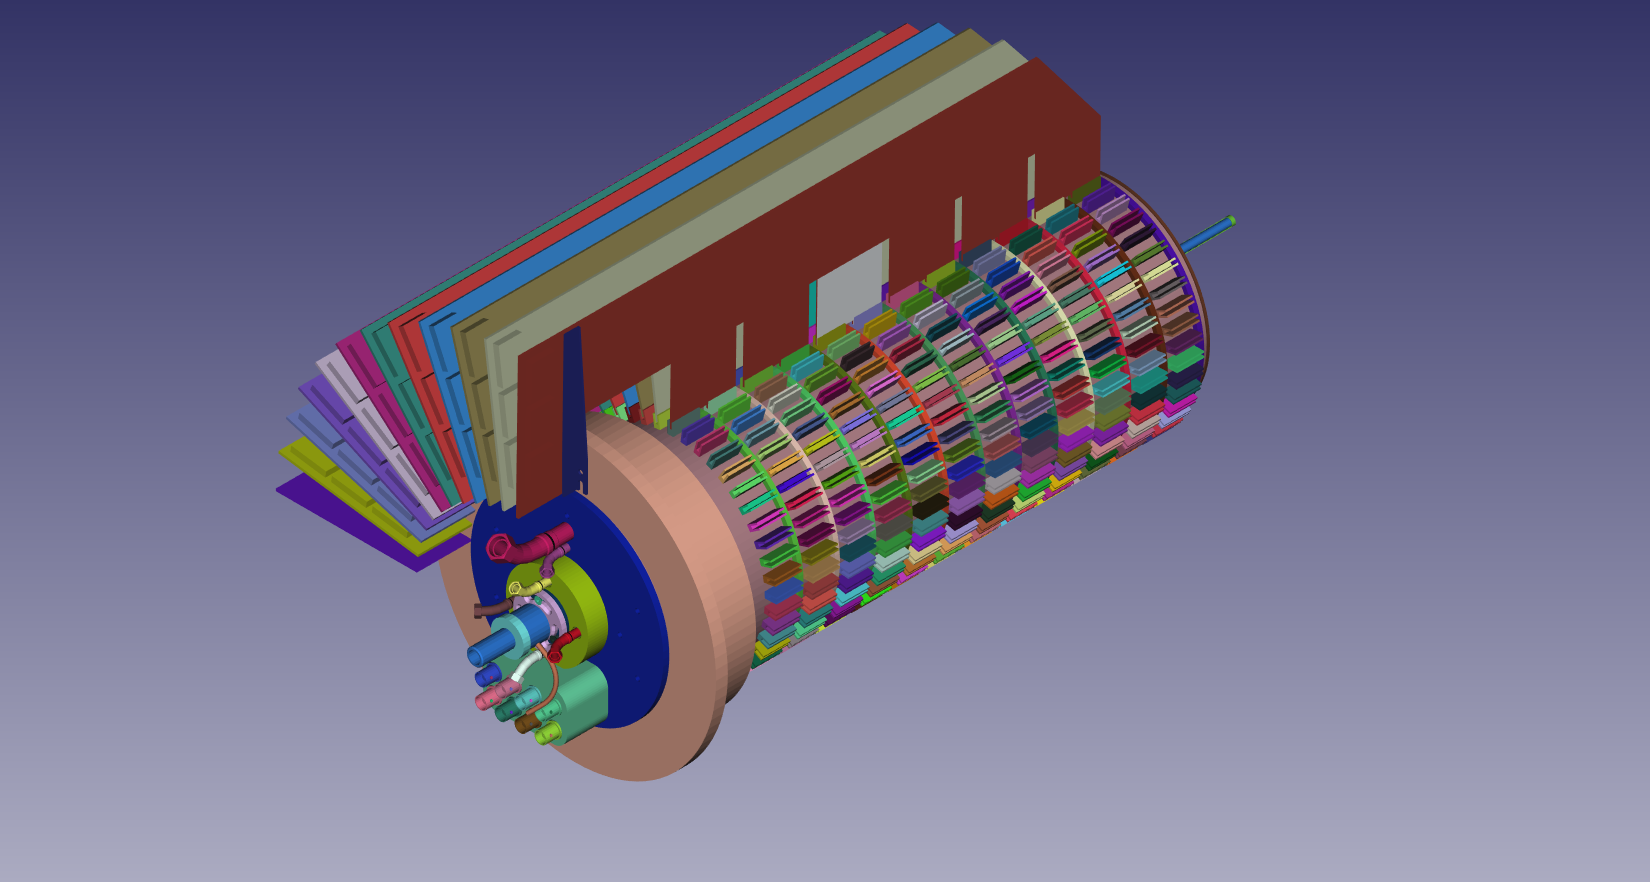
\includegraphics[angle=0, width=0.45\textwidth,clip,
     trim=50mm 10mm 80mm 0mm]{figures/Bonus12_cad.png}
    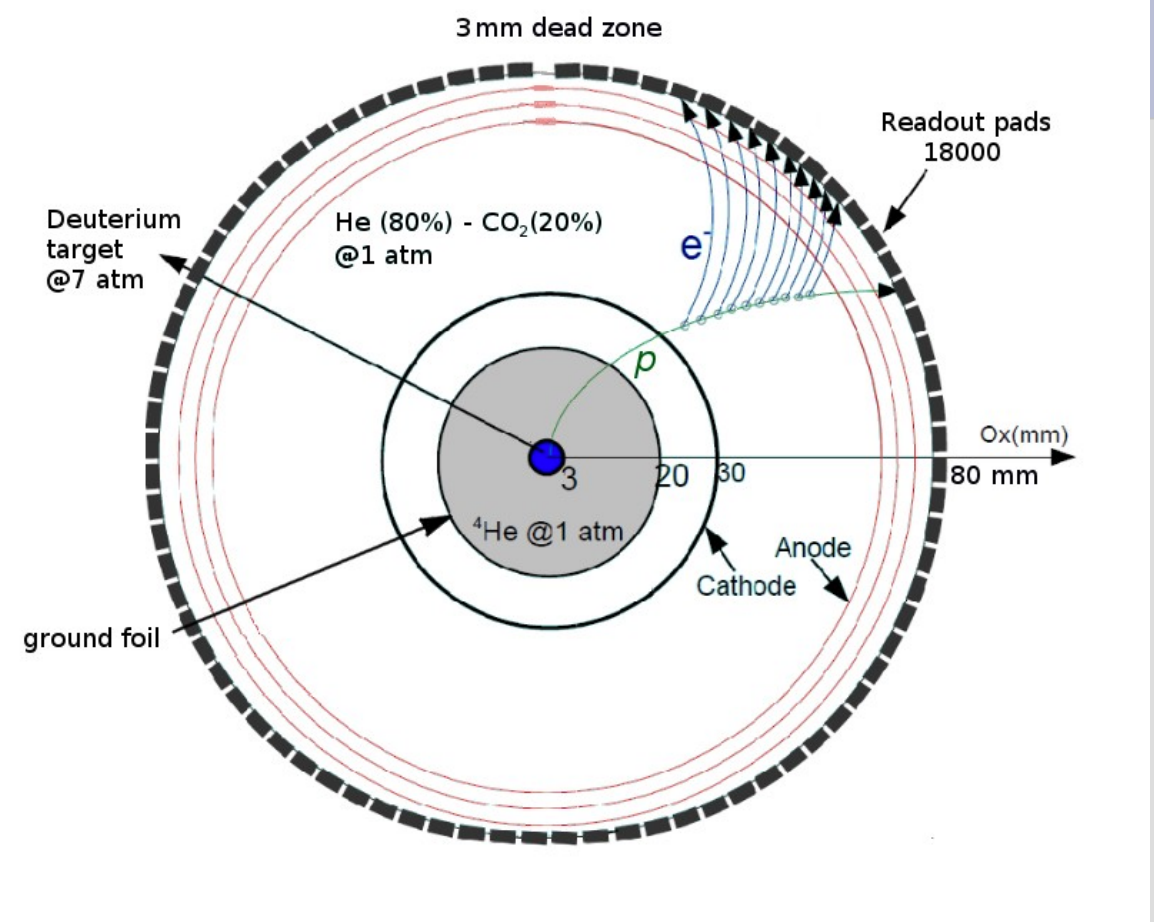
\includegraphics[angle=0, width=0.45\textwidth,clip,
     trim=0mm 10mm 20mm 0mm ]{figures/NKsBXp.png}
     \caption{(Left) Schematic layout showing BONuS12 RTPC showing the readout 
     padboard and few adaptor boards in addition to the gas lines. (Right) 
     Schematic drawing of the CLAS RTPC in a plane perpendicular to the beam 
     direction. See text for description of the elements.}
    \label{fig:bonus12}
  \end{center}
\end{figure}

The new CLAS12 RTPC (BONuS12) is 400~mm active length cylinder of 160~mm 
diameter. The electric field is directed perpendicularly to the beam direction, 
such that drifting electrons are pushed away from the beam line.  These 
electrons are amplified by three layers of cylindrical gas electron multipliers 
(GEM) and detected by the readout system on the external shell of the detector 
as illustrated in Figure~\ref{fig:bonus12}. The BONuS12 RTPC covers almost 
100\% of the azimuthal angle range.

We detail here the different regions shown in Figure~\ref{fig:bonus12} starting 
from the beam line towards larger radius:\\
\begin{itemize}
  \item The 7~atm Deuterium gas target extends along the beamline forming the 
     detector central axis. It is a 6~mm diameter aluminized Kapton straw with 
      a 62~$\mu$m wall of 492~mm length such that its entrance and exit  
      (15~$\mu$m aluminum windows) are placed outside of the detector volume.  
   The detector and the target are placed at the center of the solenoid aligned 
with the beamline.  
\item The first gas gap covers the radial range from 3~mm to 20~mm. It is 
   filled with $^{4}$He gas at 1~atm to minimize secondary interactions from
      M\o{}ller electrons scattered by the beam. This region is surrounded by a 
      6~$\mu$m thick window made of grounded aluminized Mylar.
   \item The second gas gap region extends between 20~mm and 30~mm and is 
      filled with the gas mixture of 80$\%$ $^{4}$He and 20$\%$ CO$_2$. This 
      region is surrounded by a 6~$\mu$m thick window made of aluminized Mylar.
   \item The drift region is filled with the same $^4$He-CO$_2$ gas mixture and 
      extends from the cathode to the first GEM, 70~mm away from the beam axis.  
     
   \item The electron amplification system is composed of three GEMs located at 
   radii of 70, 73, and 76~mm.  

   \item The readout board has an internal radius of 79~mm and collects charges 
      after they have been multiplied by the GEMs. The board has a total of 
      17280 pads (=180 (in $\phi, \Delta \phi = 2^{\circ}$)~$\times$ 96 (in z, 
      $\Delta$z= 4mm). Adaptor and protection circuit boards are plugged 
      directly on the outer side and transmit the signal to the Hitachi cables 
      connected to the standard MVT DREAM electronics.
\end{itemize}



\section{BONuS12 in CLAS12 Coordinates}

The center of the BONuS12 RTPC will be aligned with the center of the solenoid, 
which is 1.303 m to the left of Hall-B center. Figure~\ref{fig:bonus12-hallb} 
shows the detailed coordinates of all the beamline elements in RG-F with 
respect to Hall-B's center. Figure~\ref{fig:bonus12-zoom} presents the geometry 
and the coordinates of the BONuS12 RTPC, the FMT, and the Moller cone with 
respect to the center of the solenoid.  


The geometry database will contain 6 parameters to describe the actual location 
of the RTPC relative to this ideal setup:
\begin{itemize}
   \item Displacements in $x$, $y$, and $z$ in mm.
    \item Pitch ($\frac{\Delta y}{\Delta z}$), yaw ($\frac{\Delta x}{\Delta 
       z}$), and roll ($\Delta \phi$ between the zero-degree mark on the 
       padboard, its seam, and the $\phi$= 0 direction in the CLAS12 coordinate 
       system, beam left pointing to sector 1).
\end{itemize}


\begin{figure}[h!]
  \begin{center}
    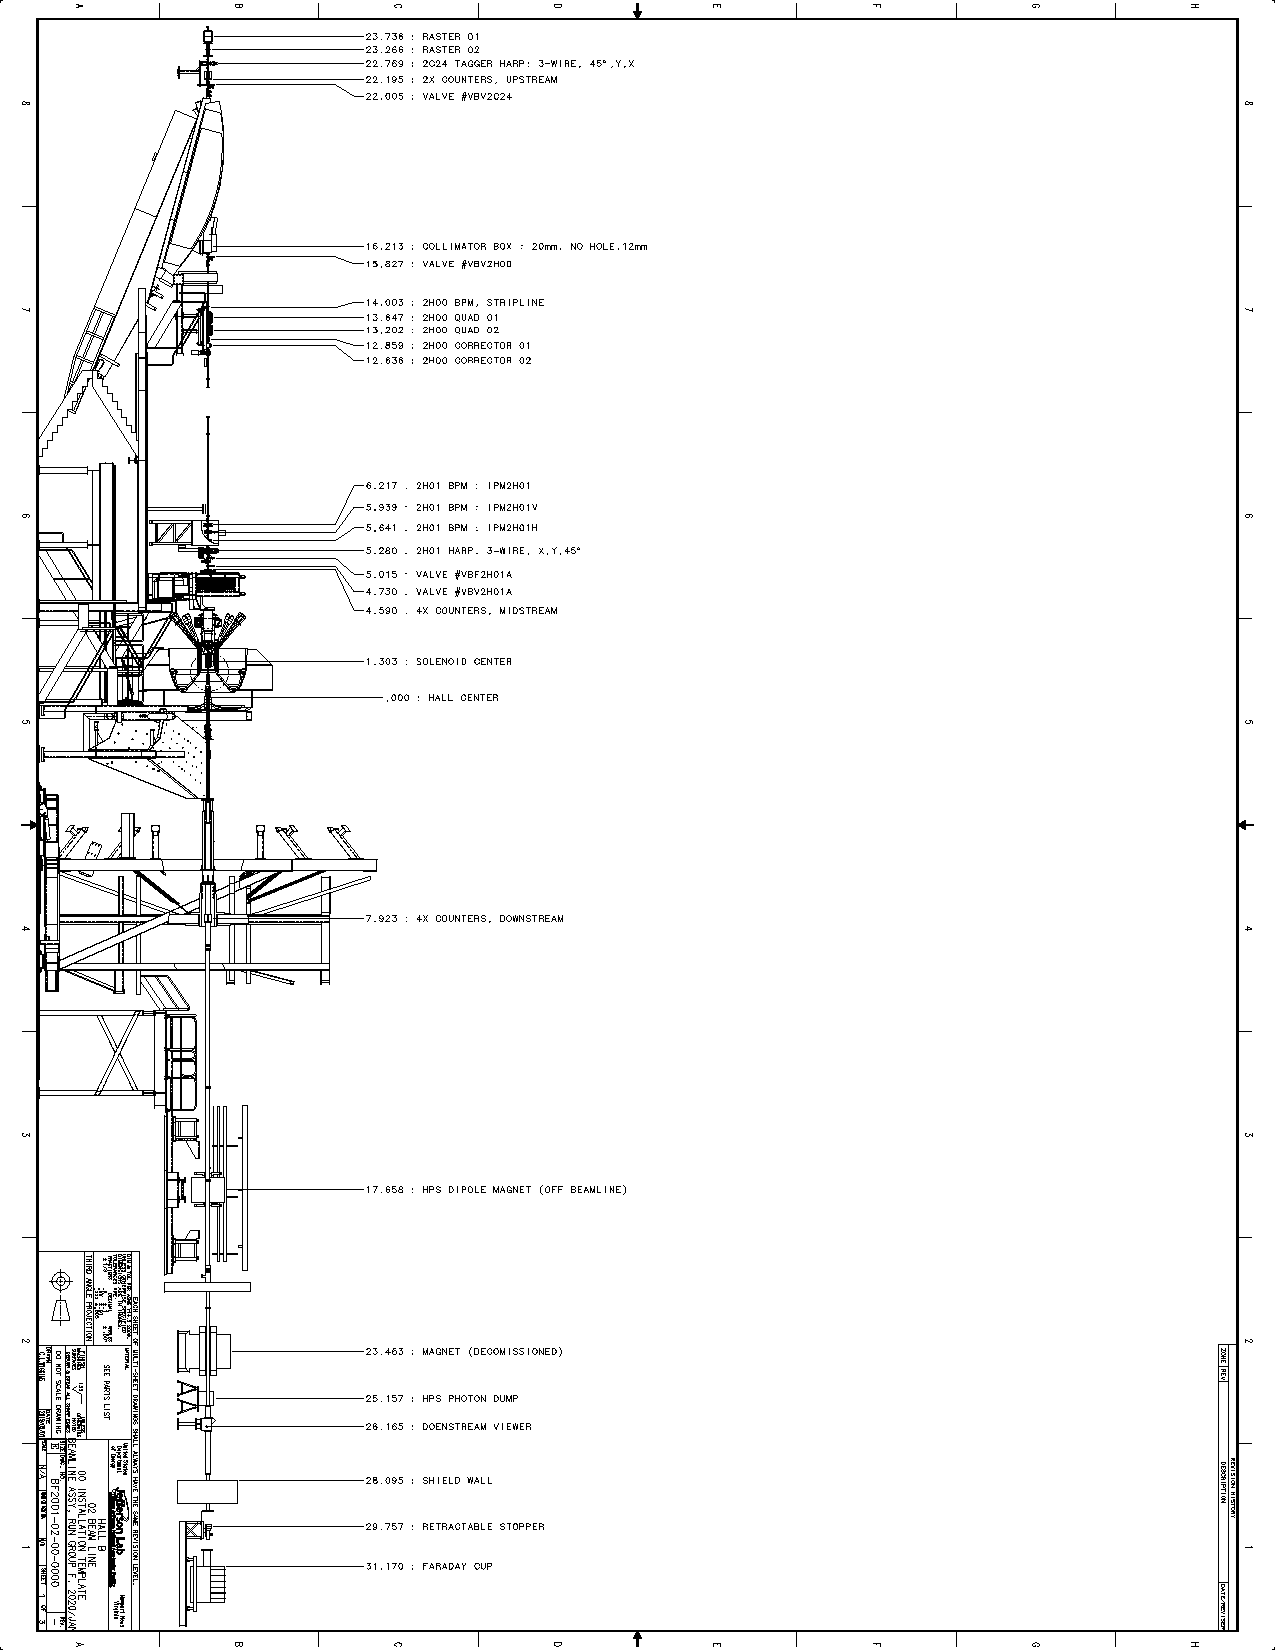
\includegraphics[angle=-90, width=0.7\textwidth,clip,
     trim=0mm 0mm 0mm 300mm]{figures/BF2001-02-00-0000_-_PDF.pdf}
     \caption{Beamline drawing showing the coordinates of all the beamline 
     elements with respect to the center of Hall-B in RGF setup.}
    \label{fig:bonus12-hallb}
  \end{center}
\end{figure}


\begin{figure}[h!]
  \begin{center}
    \includegraphics[page=2, width=1.0\textwidth,clip,
     trim=0mm 0mm 0mm 0mm]{figures/BF2001-02-00-0000_-_PDF.pdf}
     \caption{Beamline drawing showing the coordinates of the BONuS12 RTPC, 
     FMT, and the Moller cone with respect to the center of the solenoid.}
    \label{fig:bonus12-zoom}
  \end{center}
\end{figure}






\end{document}


